\documentclass{beamer}
\usetheme{Boadilla}

\usepackage{amsmath}
\usepackage{amsfonts}
\usepackage{hyperref}
\usepackage{biblatex}
\graphicspath{ {./images/} }


\title{Knowledge Transfer via Dense Cross-Layer Mutual-Distillation}
\author{Ksenofontov Gregory}
\institute{MIPT}


\begin{document}

\begin{frame}
    \titlepage
\end{frame}

\begin{frame}{KD and DML}
 Given the training data $X = \{x_n\}^N_{n=1}$ of $M$ classes, with labels $Y = \{y_n\}^N_{n=1}$. $W_t$ -- a teacher network, and  $W_s$ -- a student network.
    \begin{block}{Knowledge Distillation}
        The teacher network $W_t$ is pretrained and fixed. The student network is trained by minimizing
        $$L_s = L_c(W_s, X, Y) + \lambda L_{kd}(\hat P_t, \hat P_s), $$
        where $L_{kd}$ -- cross entropy 
        $$L_{kd}(\hat P_t,\hat P_s) = − \frac1N \sum^N_{n=1}\sum^M_{m=1} \hat P^m_t(x_n) \log\hat P^m_s (x_n)$$
        and $\lambda$ -- a balancing coefficient
    \end{block}
\end{frame}

\begin{frame}{KD and DML}
 Given the training data $X = \{x_n\}^N_{n=1}$ of $M$ classes, with labels $Y = \{y_n\}^N_{n=1}$. $W_t$ -- a teacher network, and  $W_s$ -- a student network.
    \begin{block}{Deep Mutual Learning}
        The teacher network $W_t$ and the student network are trained by jointly minimizing
        $$L_s = L_c(W_s, X, Y) + \lambda L_{dml}(\hat P_t, \hat P_s)$$
        $$L_t = L_c(W_t, X, Y) + \lambda L_{dml}(\hat P_s, \hat P_t), $$
        where $L_{dml}$ -- KL divergence (relative entropy)
        $$L_{dml}(\hat P_t,\hat P_s) = − \frac1N \sum^N_{n=1}\sum^M_{m=1} \hat P^m_t(x_n) \log\frac{\hat P^m_t (x_n)}{\hat P^m_s (x_n)}$$
        and $\lambda$ -- a balancing coefficient
    \end{block}
\end{frame}

\begin{frame}{KD and DML}
Authors of the article proposes a new method \textbf{Dense Cross-layer Mutual-distillation (DCM)}, that enhances DML via jointly addressing two issues listed below.
    \begin{enumerate}
        \item The information contained in the hidden layers of networks has not been explored
        \item The problem of connecting more effective knowledge representation learning
    \end{enumerate}
\end{frame}

\begin{frame}{DCM}
Given the training data $X = \{x_n\}^N_{n=1}$ of $M$ classes, with labels $Y = \{y_n\}^N_{n=1}$. $W_t$ -- a teacher network, and  $W_s$ -- a student network.\par
    \begin{block}{Dense Cross-layer Mutual-distillation}
        Let Q = $\{(t_k, s_k)\}^K_{k=1}$ -- set of $K$ pairs of the same-staged layer indices of the teacher network $W_t$ and the student network $W_s$, indicating the locations of auxiliary classifiers ($(t_{K+1}, s_{K+1})$ -- default classifier). DCM simultaneously minimizes the following two objectives
        $$L_s = L_c(W_s, X, Y) + \alpha L_{ds}(W_s, X, Y ) + \betha L_{dcm1} (\hat P_t, \hat P_s) + \gamma L_{dcm2} (\hat P_t, \hat P_s)$$
        $$L_t = L_c(W_t, X, Y) + \alpha L_{ds}(W_t, X, Y ) + \betha L_{dcm1} (\hat P_s, \hat P_t) + \gamma L_{dcm2} (\hat P_s, \hat P_t),$$
    \end{block}

\end{frame}

\begin{frame}{DCM}
    \begin{block}{$L_{ds}(W_s, X, Y)$}
        This loss denotes sum of cross-entropy losses for all auxiliary classifier
        $$L_{ds}(W_s, X, Y) = \sum_{k=1}^{K} L_c(W_s, X, Y)$$
    \end{block}
    \begin{block}{$L_{dcm}(\hat P_t, \hat P_s)$}
        This two losses in total denote sum of all KD losses of all pair combinations of classifiers
        $$L_{dcm1}(\hat P_t, \hat P_s) = \sum_{k=1}^{K+1} L_{kd}(\hat P_{t_k}, \hat P_{s_k})$$
        $$L_{dcm2}(\hat P_t, \hat P_s) = \sum_{i,j=1; i\neq j}^{K+1} L_{kd}(\hat P_{t_i}, \hat P_{s_j})$$
    \end{block}
\end{frame}

\begin{frame}{DCM algorithm}
    \begin{figure}[h]
        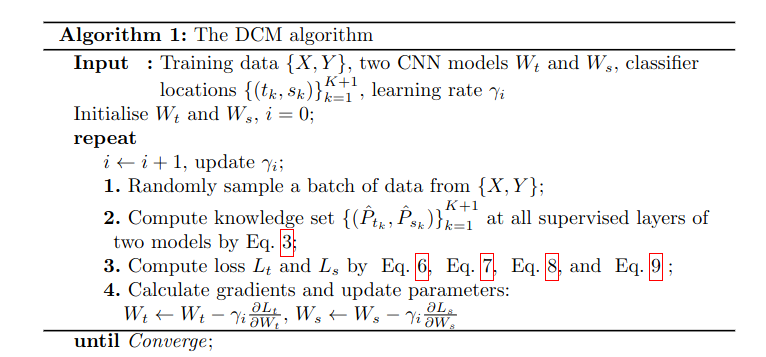
\includegraphics[scale=0.45]{images/algo.png}
     \end{figure}
\end{frame}

\begin{frame}{Setting of $Q$}
    \begin{enumerate}
        \item \textit{Where to place auxiliary classifiers?}
        Use a \textbf{practical} principle, adding auxiliary classifiers merely to down-sampling layers of a backbone network
        \item \textit{How to design structures of auxiliary classifiers?}
        Use a \textbf{heuristic} principle, making the paths from the input to all auxiliary classifiers have the same number of downsampling layers as the backbone network and using backbone’s building blocks
    \end{enumerate}
\end{frame}

\begin{frame}{Main experiments}
    \begin{figure}[h]
        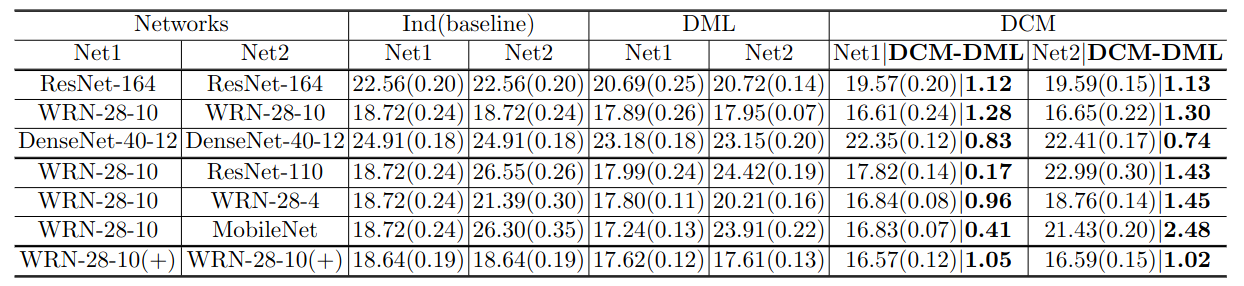
\includegraphics[scale=0.25]{images/table1.png}
     \end{figure}
\end{frame}

\begin{frame}{Setting of $Q$ experiments}
    \begin{enumerate}
        \item \textit{Where to place auxiliary classifiers?}
            \begin{figure}[h]
                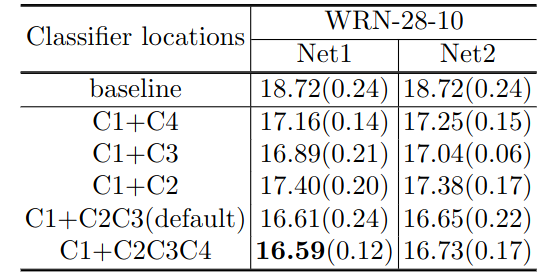
\includegraphics[scale=0.25]{images/table3.png}
            \end{figure}
        \item \textit{How to design structures of auxiliary classifiers?}
            \begin{figure}[h]
                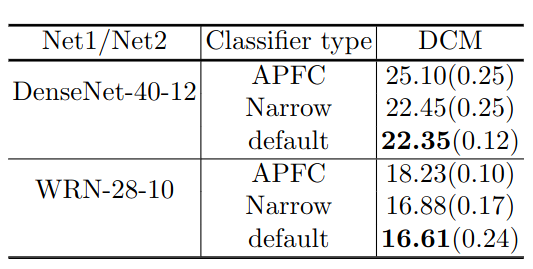
\includegraphics[scale=0.25]{images/table4.png}
            \end{figure}
    \end{enumerate}
\end{frame}

\begin{frame}{Loss experiments}
    \begin{figure}[h]
        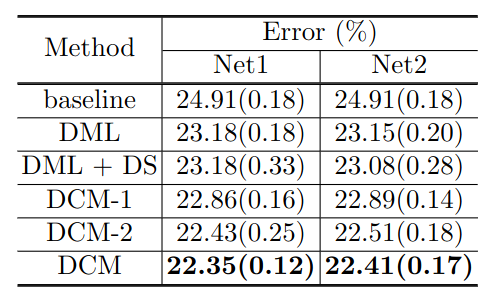
\includegraphics[scale=0.4]{images/table5.png}
    \end{figure}
\end{frame}

\begin{frame}{Noise experiments}
    \begin{figure}[h]
        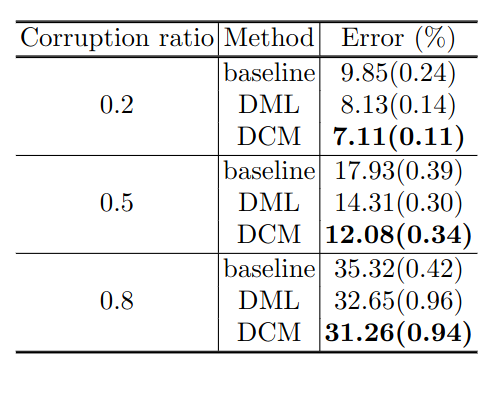
\includegraphics[scale=0.4]{images/table7.png}
    \end{figure}
\end{frame}


\end{document}
